\section{考察}
\label{sec:kousatsu}

本システムは，高い没入感を得るために「ユーザの能動的操作」があり，かつ「空間的なフィードバック」があるシステムの作成を目的として設計・評価を実施した．本節では，\ref{sec:hyouka}節で示した単体テストおよび結合テストの結果に基づく考察を行い，実装・評価を通じて確認された本システムのハードウェア依存性を整理した後，評価指標そのものがシステムの有意性を議論する指標として妥当であるかを検討する．続いて，既存システムとの比較および本システムの優位点を整理し，\ref{sec:ketsugo_result}項の末尾で示したハッカソン参加者共通アンケートの結果に基づく考察を行う．本稿の評価は，システムが設計通り動作することを確認する技術的評価（結合テスト）と，利用者からどのように評価されたかを示す主観評価（参加者共通アンケート）の二段階で構成されており，本節ではこの2つを統合して本システムの有効性を検討したうえで，最後に改善案と今後の展望について述べる．

\subsection{単体テストおよび結合テストの結果に関する考察}
\label{sec:kousatsu_test}

\subsubsection{同期確立時間の増大とその要因分析}
\label{sec:kousatsu_douki}

結合テストにおいて，同期開始条件を\SI{50}{ms}以下とした場合，一度同期が確立した後の楽器間の演奏ズレはハース効果\cite{haas1951}に基づくMOPの目標値である\SI{50}{ms}未満に収まった．一方，同期の確立自体に要する時間（ボタン押下から楽曲再生開始までの応答遅延）は，全53回の試行のうち8回がTanらの示す\SI{60}{s}\cite{tan2026}の閾値を超過し，成功率は84.9\%にとどまった．

この2つの同期開始条件の差を比較するため，表\ref{tab:song_start_60ms}および表\ref{tab:song_start_50ms}の測定値をBPM別に図示したものを図\ref{fig:sync_condition_compare}に示す．図\ref{fig:sync_condition_compare}(a)より，\SI{50}{ms}条件の平均応答遅延は全てのBPMで\SI{60}{ms}条件を上回り，標準誤差（エラーバー）も大きい．すなわち，同期開始条件の厳格化は応答遅延を平均的に増大させるだけでなく，試行ごとのばらつきも拡大させている．また，図\ref{fig:sync_condition_compare}(b)より，\SI{60}{s}以内に楽曲再生が開始された試行の割合は\SI{60}{ms}条件では全BPMで100\%である一方，\SI{50}{ms}条件ではBPM60・90・150で低下しており，特にBPM150では50.0\%まで低下した．ただし，同条件の試行数は10回と少なく，BPMに対して単調な傾向も見られないことから，BPMに固有の要因であるかは判別できない．この未達成の要因として，技術的観点から次の2点が考えられる．

\begin{figure}[htbp]
  \centering
  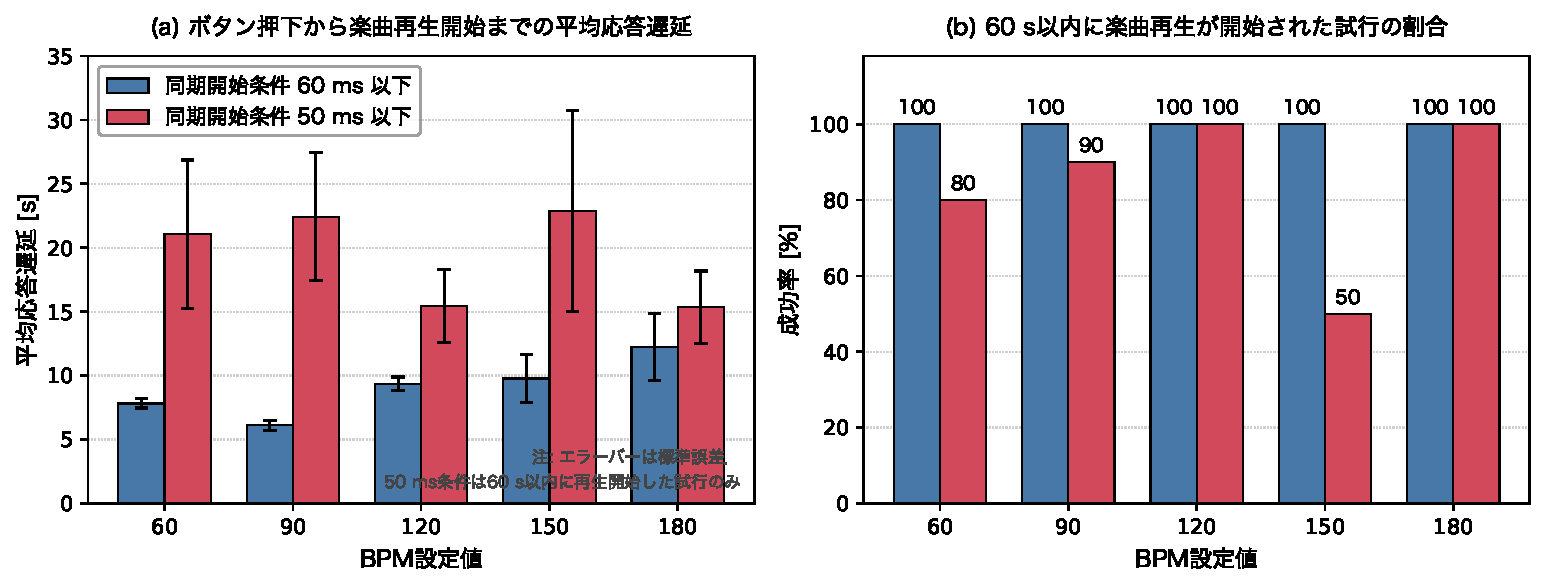
\includegraphics[width=\textwidth]{figs/sync_condition_compare.pdf}
  \caption{同期開始条件（\SI{60}{ms}以下・\SI{50}{ms}以下）別のボタン押下から楽曲再生開始までの応答遅延と成功率の比較}
  \label{fig:sync_condition_compare}
\end{figure}

第一に，同期補正ループの収束特性と許容閾値の関係である．\ref{sec:gakki_naibu}項で述べた通り，本システムの同期確立は，マスターと各スレーブが'R'通信で演奏位置のずれ（diff）を交換し，補正を繰り返した結果，「接続中の全楽器のずれが閾値以内」という条件が成立した時点で完了する．このずれの測定には，往復遅延の半分を片道遅延とみなす近似が用いられているため，測定値には無線通信の遅延変動に由来する誤差が含まれる．許容閾値を\SI{50}{ms}に狭めると，この測定誤差やパケットロスによるずれの揺らぎが閾値幅に対して相対的に大きくなり，全楽器のずれが同時に閾値内へ収まる事象が生じにくくなるため，条件成立までの時間が延びたと考えられる．また，2.4GHz帯の混雑によるUDPパケットロスは，'R'・'O'通信の欠落として補正の機会そのものを減少させる．本テストの実施環境は実演を行ったハッカソン会場そのものではないが，いずれも大学構内という多数のWi-Fi機器が2.4GHz帯を共有する電波環境である点は共通しており，パケットロスが同期確立を遅延させた要因として十分に考えられる．なお，指揮デバイスが指令送信時に行う3周の冗長送信（周間\SI{20}{ms}，\ref{sec:siki_naibu}項）は，演奏開始・終了等の指令を送る一度きりの処理であり，同期確立の補正ループには関与しないため，同期確立時間の増大要因ではない．

第二に，中継機デバイスの回転速度の変動である．\ref{sec:gakki_naibu}項で述べた通り，各楽器デバイスはレーザー光の受光間隔からBPMを推定しており，同期確立の前提として受光間隔が安定している必要がある．しかし，\ref{sec:jissou_kan}項で述べた通り，同一のPWM設定値に対するモータの回転速度は電源電圧の変動等により試行ごとに変動し，さらに\ref{sec:kousatsu_hw}項で述べる光学系の物理的条件によって受光の成立自体が変動する．受光間隔が揺らぐとBPM推定の安定判定に時間を要するため，同期確立時間の試行間のばらつきに寄与したと考えられる．

以上より，\SI{50}{ms}という同期開始条件下での応答遅延の未達成は，ずれ測定の誤差・パケットロスの下で狭い許容閾値を全楽器同時に満たすことの難しさ，および回転速度・受光の物理的な変動に起因するものと考えられる．なお，同期開始条件を\SI{60}{ms}以下に緩和した場合は全25回の試行で成功率100\%，平均応答遅延$\SI{9054.0}{ms}$であり，許容ズレをわずか\SI{10}{ms}緩和するだけで同期確立が安定することから，本システムの同期性能は\SI{50}{ms}という閾値の近傍で動作していると言える．

\subsubsection{ユーザの能動的操作を支える処理成功率の要因分析}
\label{sec:kousatsu_sousa}

ボタン押下による操作反映の成功率は，全160回の試行のうち158回の成功で98.8\%であり，MOPの目標値である99.0\%以上にわずかに届かなかった．失敗した2回の試行はいずれも，モータドライバは動作していたにもかかわらず観覧車が回転しなかった事例である．この要因として，ブレッドボード上の配線の接触不安定が挙げられる．モータドライバまでの信号伝達は正常であったことから，ドライバ出力からモータまでの経路，すなわちブレッドボードのコンタクト部における接触抵抗の一時的な増大により，モータの起動トルクに必要な電流が供給されなかった可能性が高い．また，チャタリング防止のために設けた押下検知後の\SI{300}{ms}の待機処理（\ref{sec:siki_naibu}項）は，待機中の再押下を検出しないため，利用者が短い間隔で操作した場合に微小な検出漏れを生じさせる余地がある．

一方，指揮デバイスの振り動作によるBPM・音量変更の反映成功率は100\%であり，全試行において意図した段階が正しく反映され，多重検知や停止状態での誤反応も確認されなかった．これは，3軸加速度センサの差分算出・多重検知防止・状態反転という段階的な検知ロジック（AccManagerクラス），および可変抵抗器のアナログ値に対する移動平均処理（PotManagerクラス）が，設計通りに機能したことを示している．すなわち，ソフトウェアによる信号処理系は目標を満たす精度で動作しており，未達成の要因はブレッドボード実装というハードウェアの試作段階に固有の物理的要因に集約される．

\subsubsection{音色再現度のばらつきと合成方式の限界}
\label{sec:kousatsu_onshoku}

\ref{sec:tanka_result}項で示した通り，MOS評価に基づく音色再現度のMOP（中央値および最頻値がともに4.0以上）は全6楽器で達成された．一方，回答分布の散らばりに着目すると，ストリングス（評価4以上が90\%）に比べ，ピアノおよびキックドラム（同71\%，74\%）は第1四分位数が3であり，回答の4分の1以上が評価3以下に分布していた．この差の要因は，加算合成を基本とする本システムの音色合成方式の特性から説明できる．

ストリングスやフルートのような持続音系の楽器は，定常的な倍音構造の再現が音色の類似度を支配するため，正弦波の加算合成とビブラート・ノイズ成分の付加によって比較的高い再現度が得られる．これに対しピアノは，打鍵直後の急峻な減衰と，複数弦のわずかなピッチ差に起因するうなり（デチューン）が音色の特徴を決定づける減衰音系の楽器であり，本システムの合成方式ではこれらの時間変化の表現が不足していたと考えられる．また，キックドラムについては，音色の迫力を支配する低域（およそ\SI{100}{Hz}以下）の再生能力が使用したスピーカーの口径・筐体では不足しており，合成波形自体の問題に加えて出力系の物理的制約が評価を低下させたと考えられる．すなわち，ピアノは合成アルゴリズム上の限界，キックドラムは再生装置上の限界という，異なる技術的要因が低評価側への分布の広がりをもたらしたと整理できる．

\subsection{ハードウェア依存性に関する考察}
\label{sec:kousatsu_hw}

本節では，実装および評価の過程で確認された，本システムのハードウェア依存性について考察する．ここでハードウェア依存性とは，システムの動作や性能が，プログラムや設定値のみでは再現されず，個々のハードウェアの状態（部品の個体差，物理的な位置関係，電源の残量等）に依存する性質を指す．本システムがハードウェア依存であると考察する根拠は，次の5点である．

第一に，検知条件の設定を実施のたびにやり直す必要があったことである．\ref{sec:kan_naibu}項で述べた回転速度実測プログラム（LaserIntervalTest）は，周囲光量や取り付け誤差に対応するための適応しきい値方式を採用しているにもかかわらず，実施するごとに検知条件の設定を行う必要があった．これは，環境光・レーザーの照射位置・CdSセルの受光位置といった物理的条件が実施のたびに変化し，一度定めた設定値が再利用できないことを意味する．

第二に，レーザー光の方向と受光素子の位置関係に対する敏感さである．\ref{sec:jissou_jukou}項で述べた通り，レーザー光の方向や受光素子の微細な位置関係によって受光のしやすさが変化するため，デバイスを組み立て直すたびに発泡スチロールによる位置の微調整が必要であり，この調整の結果が同期の成立しやすさを左右した．この位置関係の敏感さを増幅させた要因が，回転部品の歪みである．3Dプリンタで製作した回転リングにはわずかな反り・歪みがあり，リングに取り付けられたレーザーモジュールの照射方向が，リングの回転位置によって変化する．このため，レーザー光の到達位置は8個のモジュール間で一意に定まらず，図\ref{fig:r_cds_angle}に示すように，受光素子側の向きを個別に傾けて合わせ込む対応が必要であった．すなわち，同期性能が光学系の物理的な組み立て状態と部品の成形精度に依存している．

\begin{figure}[htbp]
  \centering
  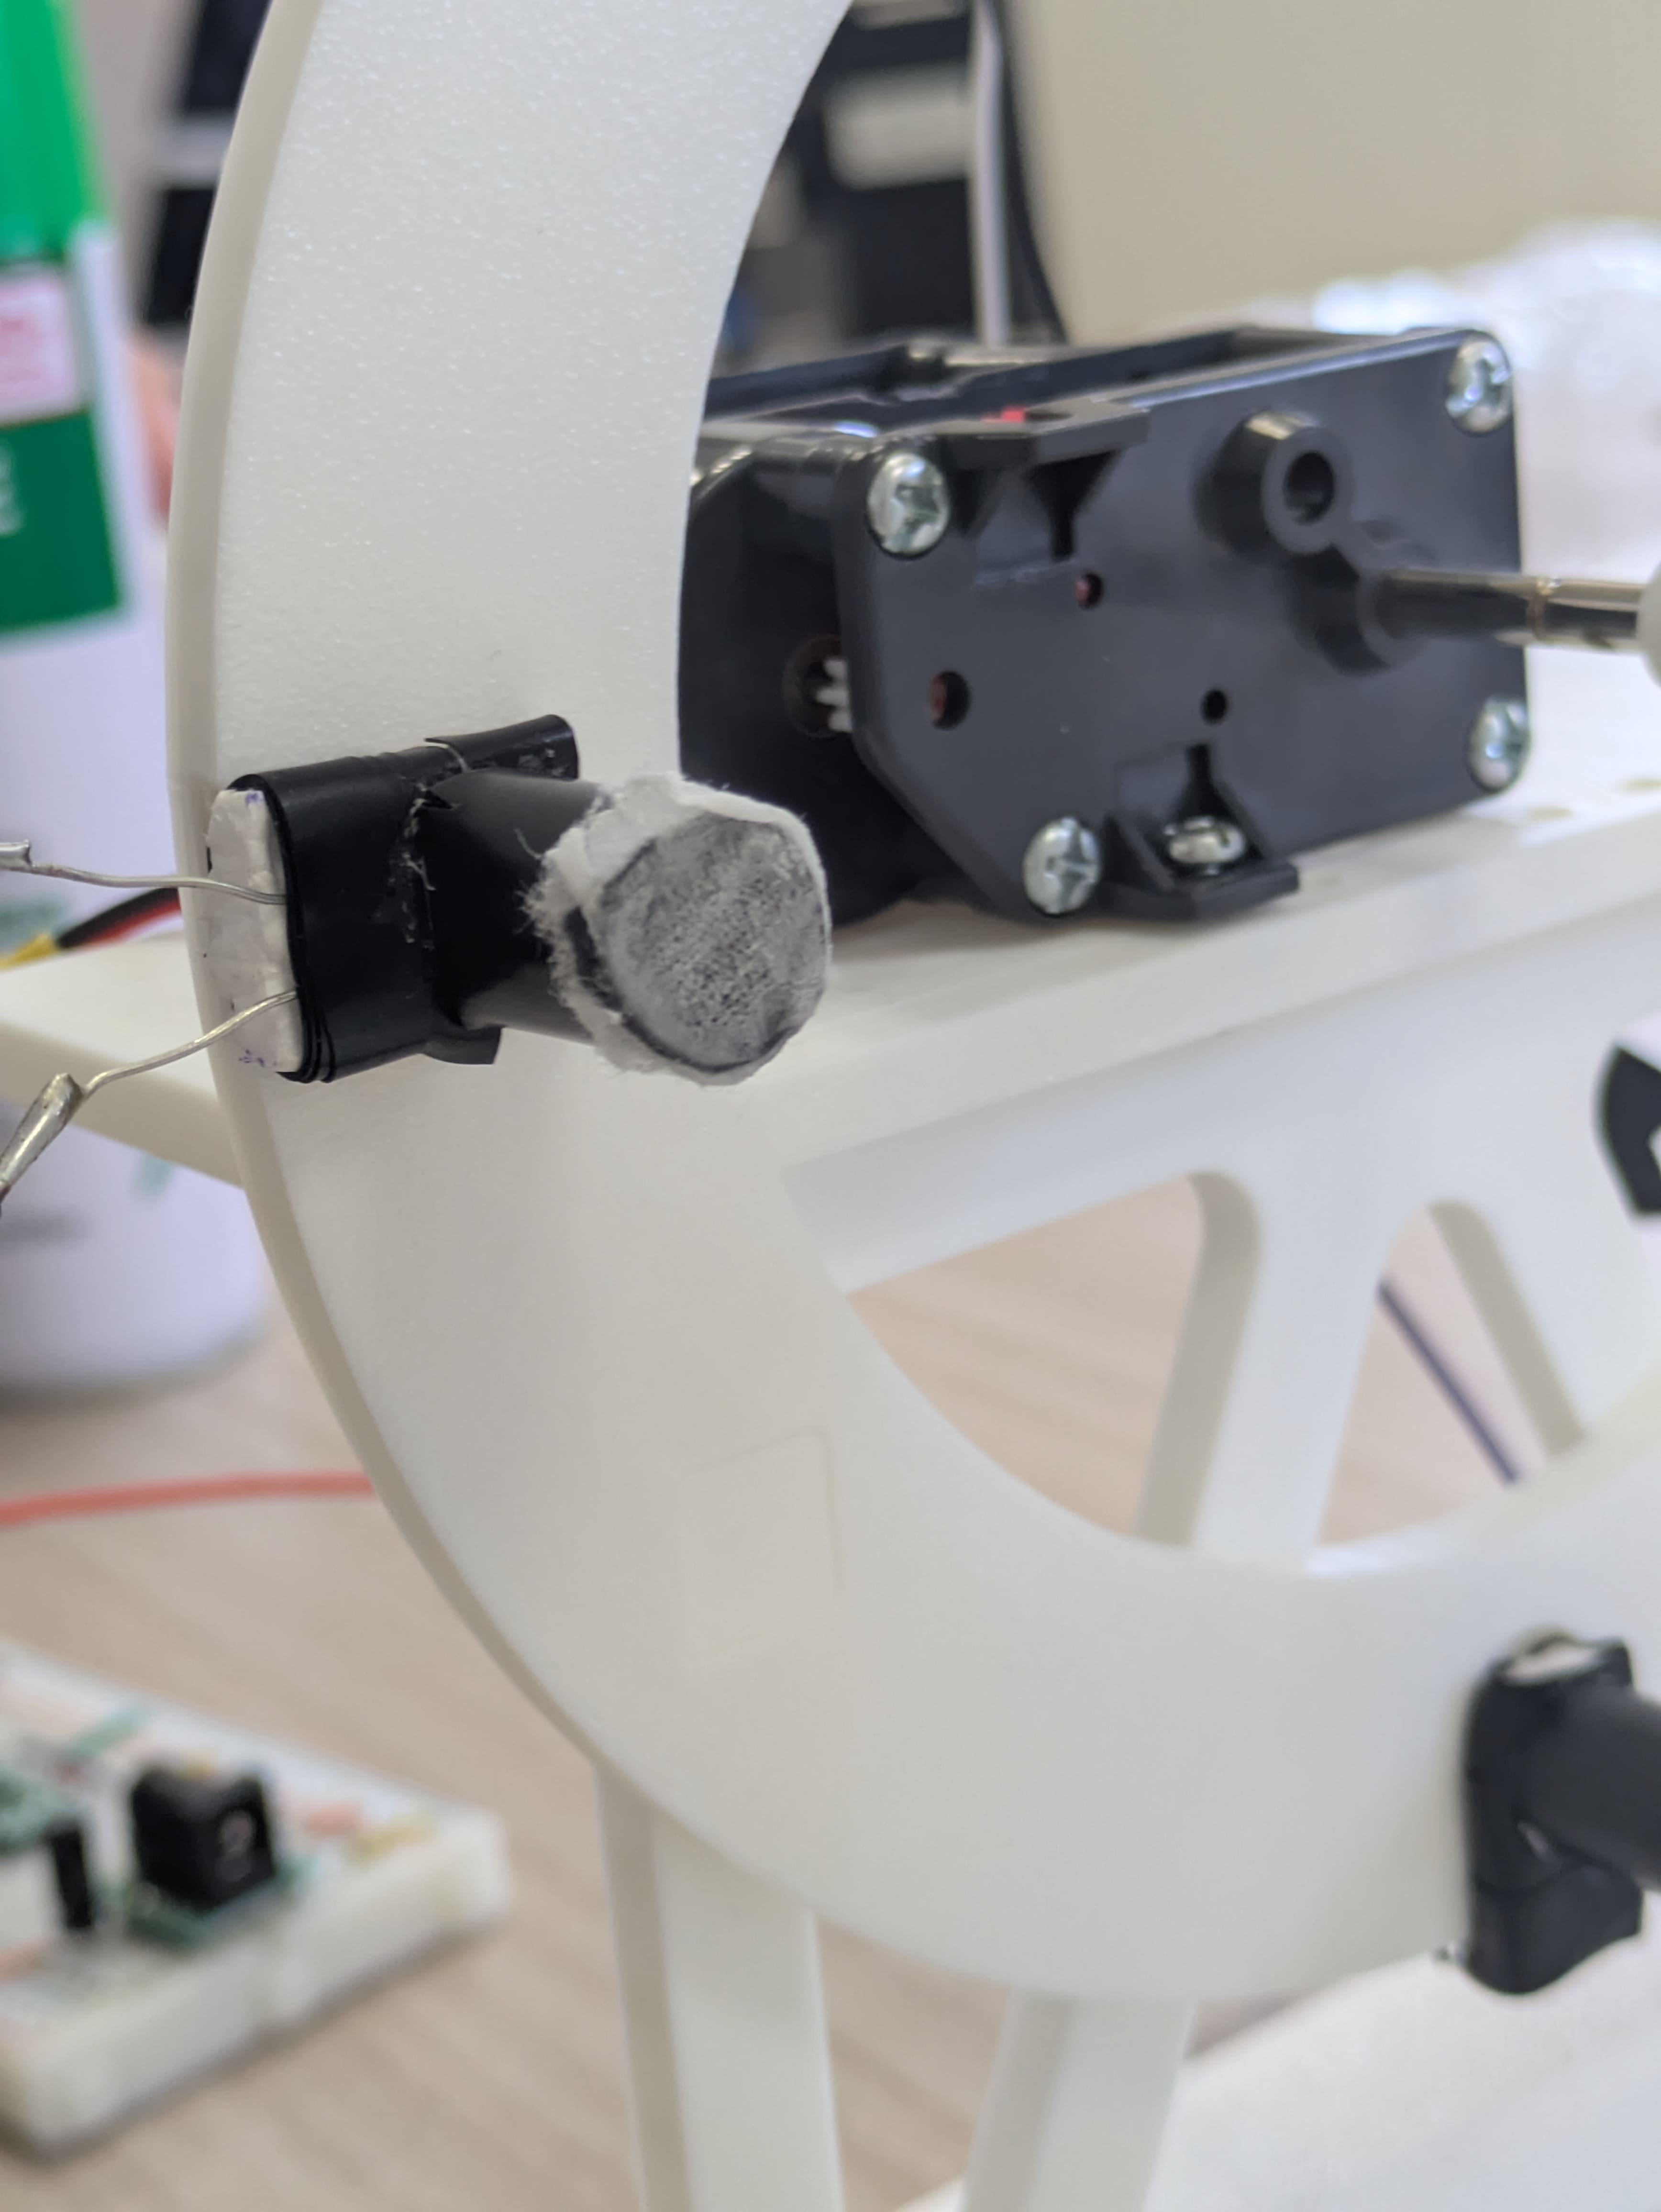
\includegraphics[width=0.55\textwidth]{figs/R_CdS.jpg}
  \caption{受光素子の取り付け角度の調整（回転部品の歪みによりレーザー光の到達方向が一定しないため，受光素子側の向きを個別に傾けて合わせている）}
  \label{fig:r_cds_angle}
\end{figure}

第三に，配線の保守性の低さである．本システムはブレッドボードとジャンパーワイヤーを多用した実装であるため，接触不良が発生した際に，多数の配線の中から断線箇所や接続ミスを特定することに時間を要した．配線経路がはんだ付けやプリント基板によって固定されていないため，故障箇所の切り分けが個々の配線の状態確認に依存する．

第四に，レーザーモジュールの光量が電池の消耗に伴い低下することである．実装では，光量の不足への対策として外部抵抗を除去し，レーザーモジュールに内蔵された回路のみで駆動する構成としたため，電池電圧の低下がそのまま光量の低下として現れる．図\ref{fig:laser_strong_weak}に示す通り，スイッチをONにした直後は受光部に明瞭な輝点が確認できる一方，時間経過後は輝点が減光しており，両者の光量の差は目視でも判別できる．光量の低下は受光時と非受光時の明暗差を縮小させるため，受光検知の成立が電池の残量という時間変化するハードウェア状態に依存する．

\begin{figure}[htbp]
  \centering
  \begin{minipage}{0.48\textwidth}
    \centering
    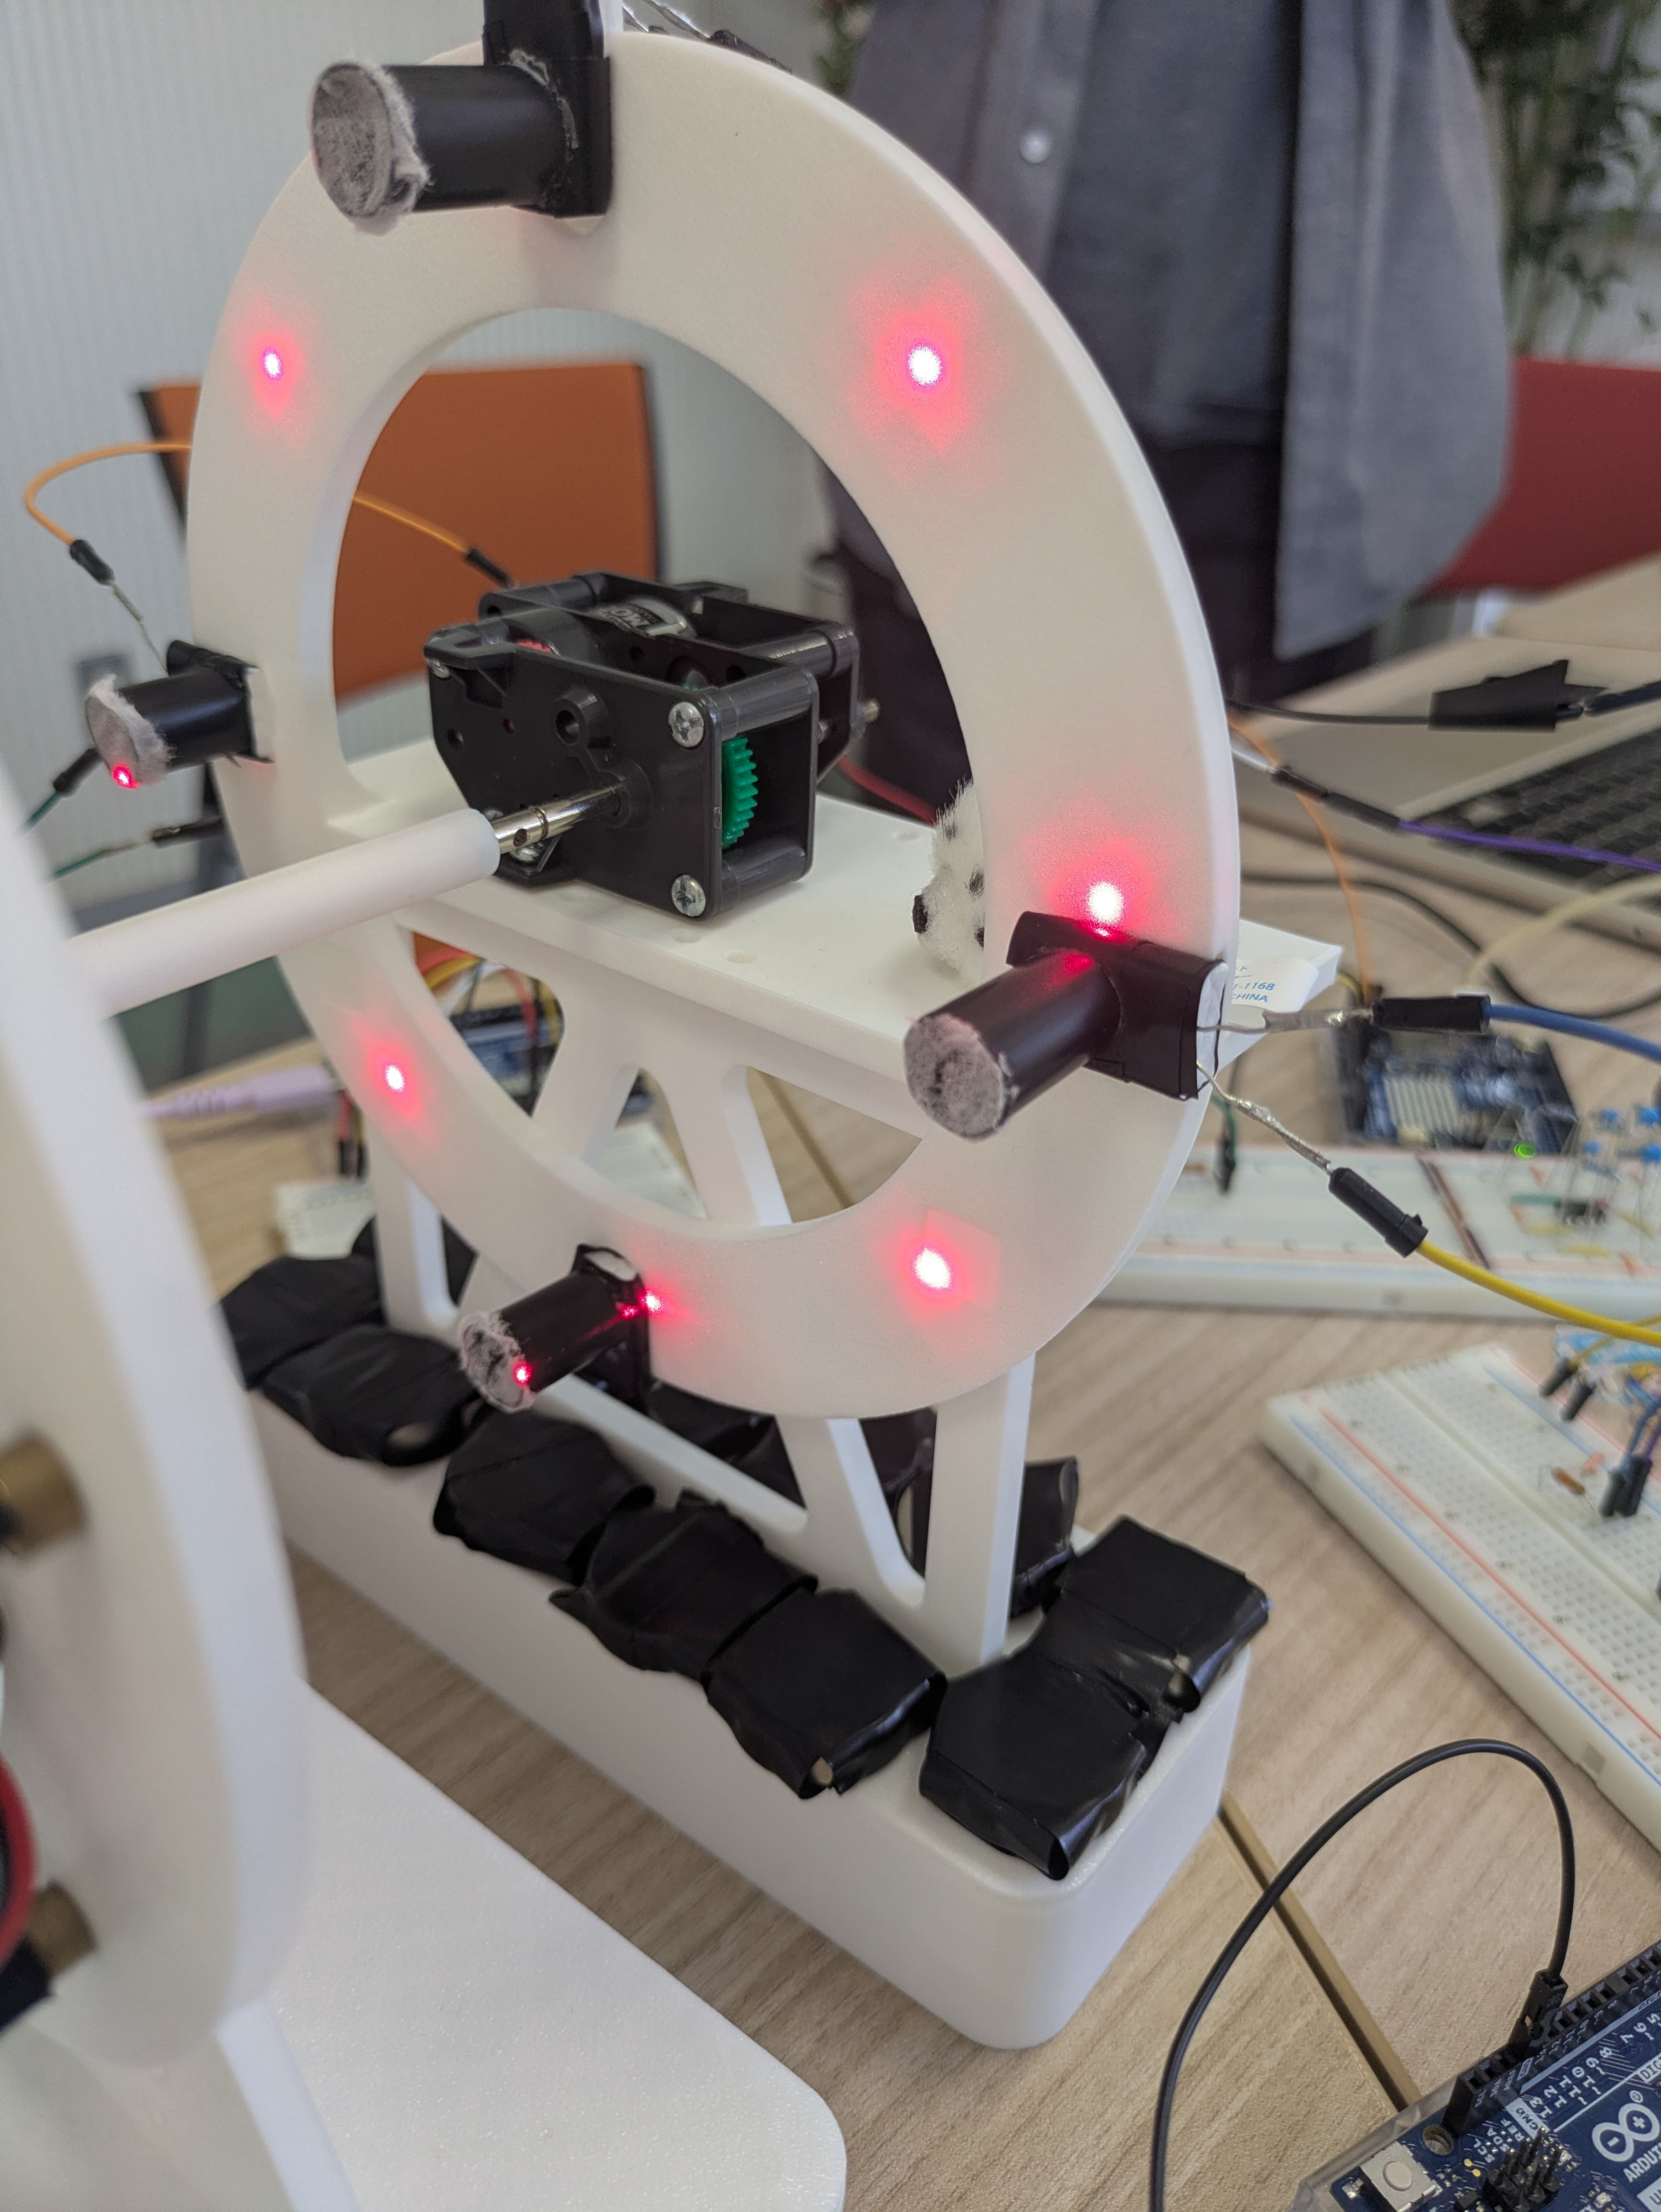
\includegraphics[width=\textwidth]{figs/strong_omote.jpg}
  \end{minipage}
  \hfill
  \begin{minipage}{0.48\textwidth}
    \centering
    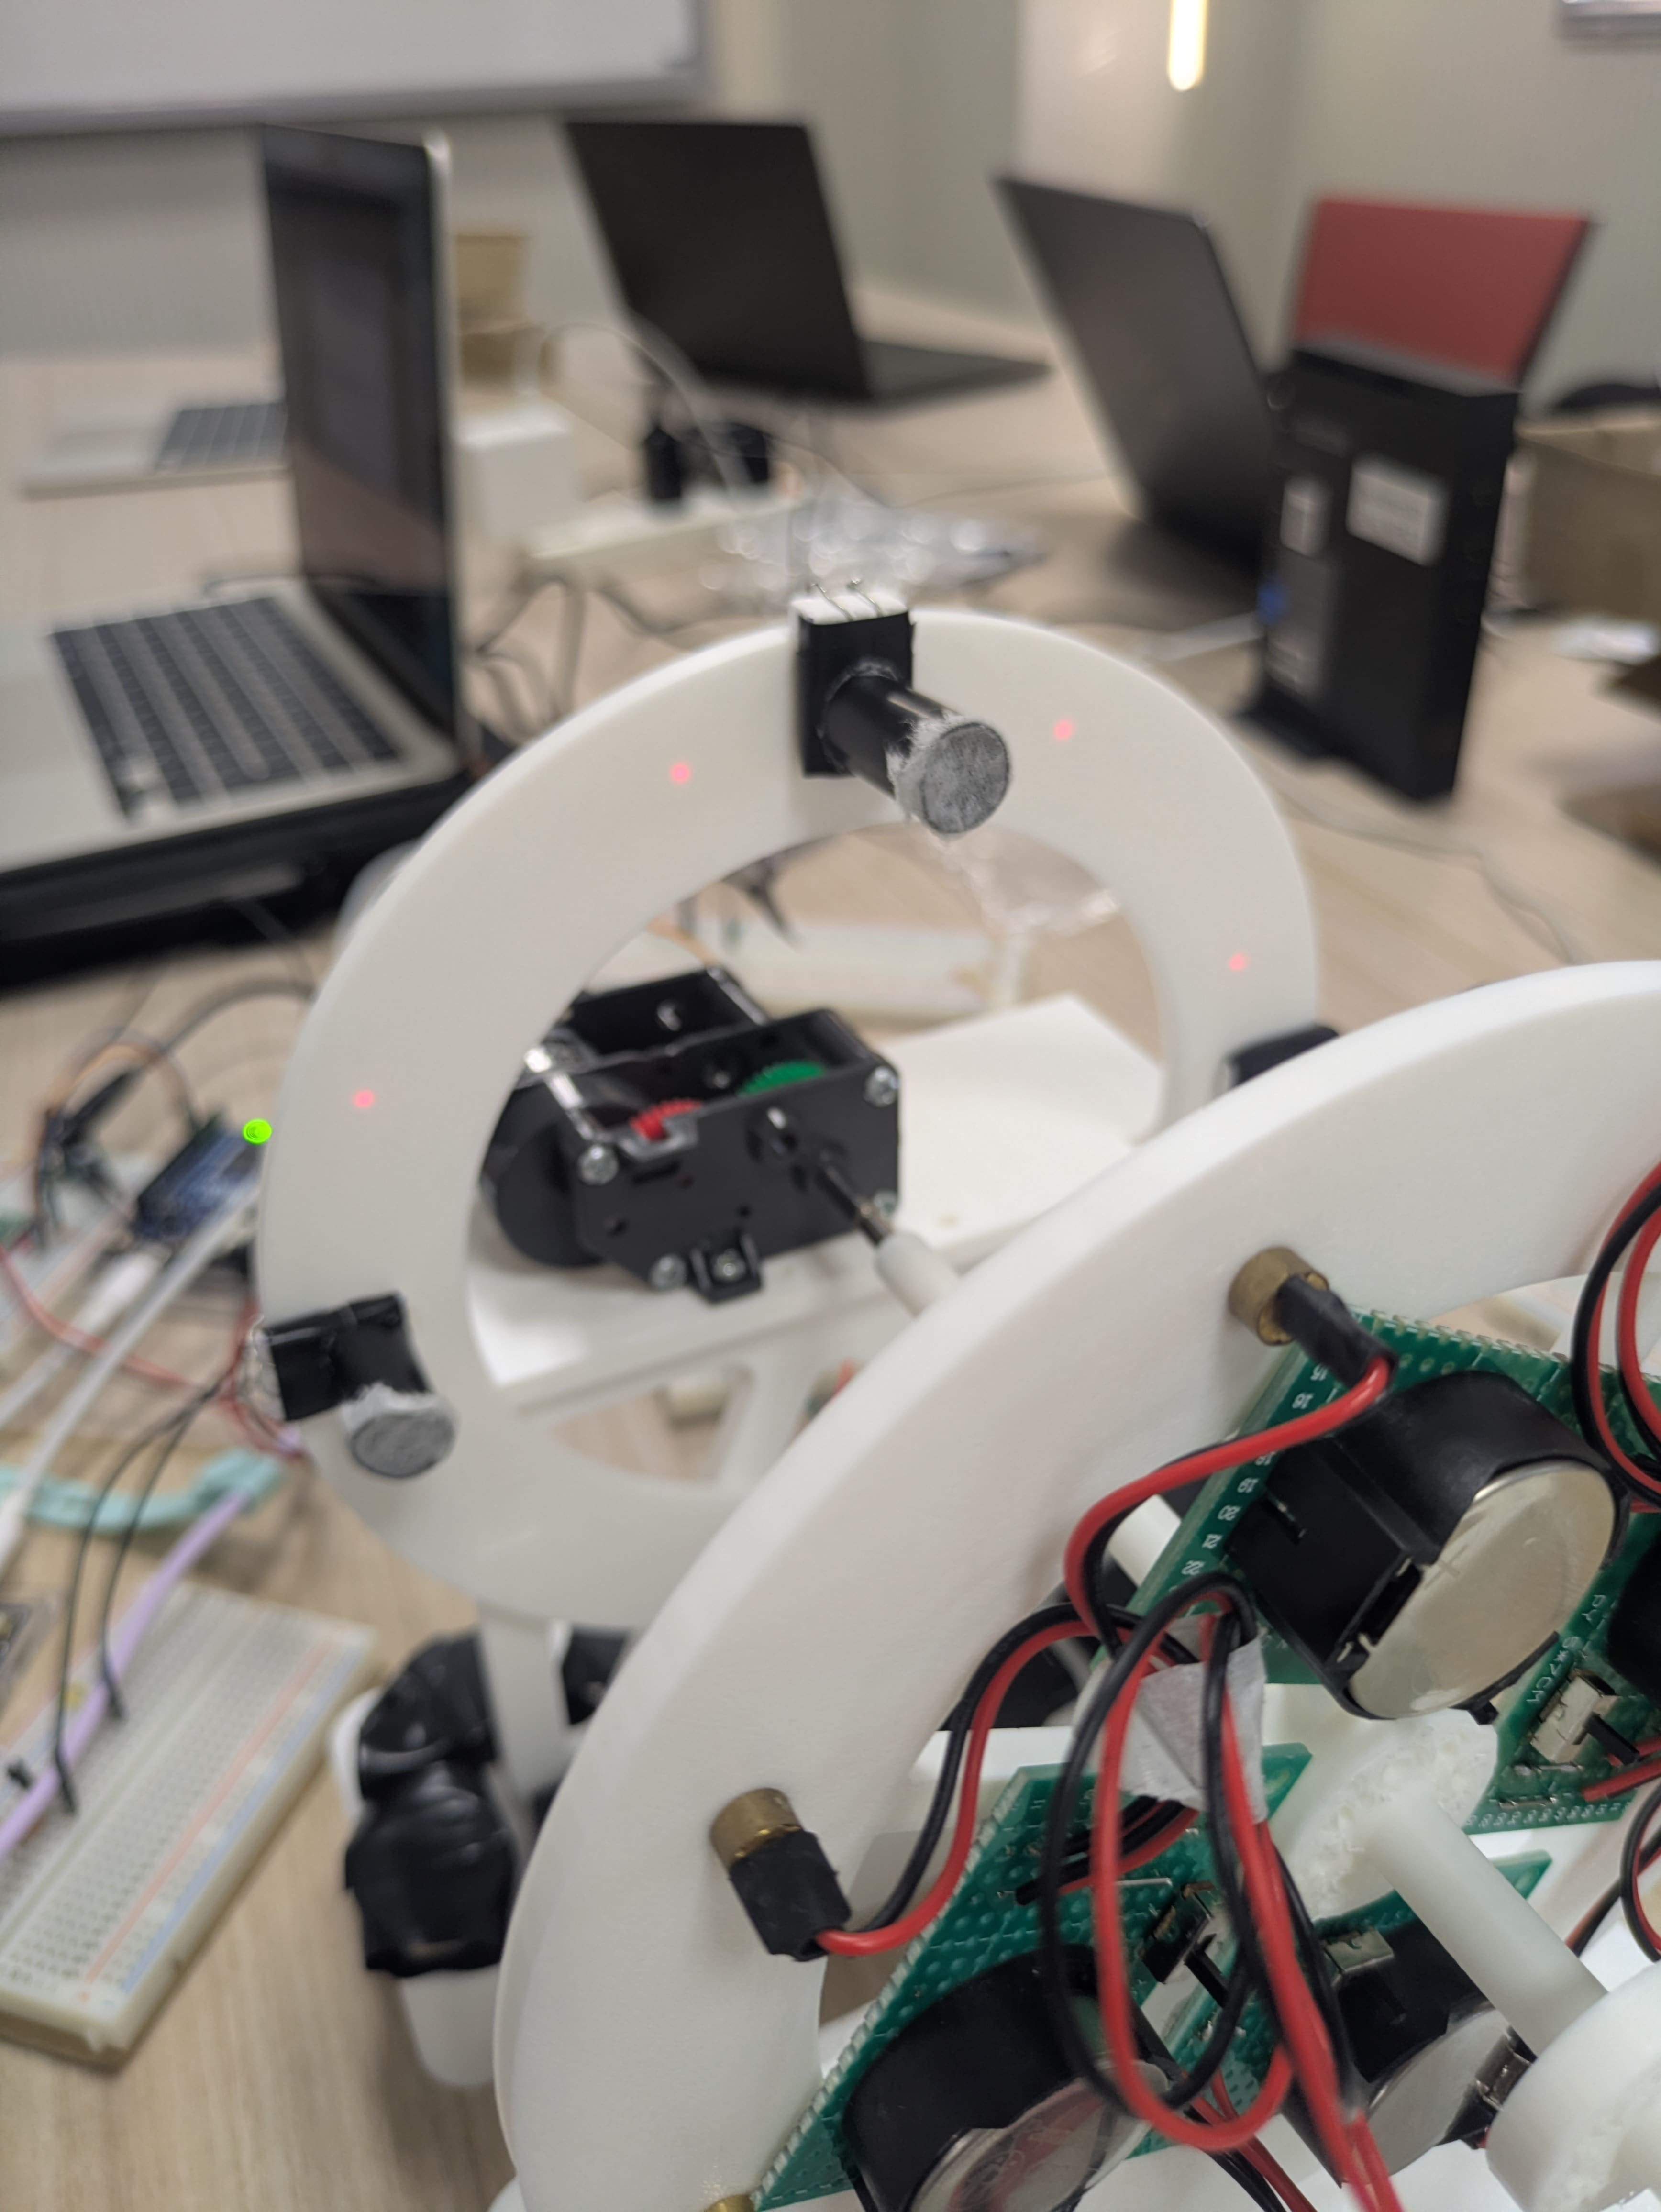
\includegraphics[width=\textwidth]{figs/weak_omote.jpg}
  \end{minipage}
  \caption{電池の消耗に伴うレーザー光量の変化（左：スイッチON直後，右：時間経過後．受光部に投影された輝点の明るさが低下している）}
  \label{fig:laser_strong_weak}
\end{figure}

第五に，ボタン電池の消耗の速さである．回転リング上の8個のレーザーモジュールを演奏中常時点灯させる構成であるため電池の消耗が早く，数時間規模の連続稼働は電池交換なしには維持できなかった．したがって，長時間の展示・実演には電池交換という人手の介入が前提となる．

以上の5点は，いずれも「同一のプログラム・同一の設定値を用いても，ハードウェアの状態が変われば同一の動作が再現されない」という共通の性質を持つ．この性質は，第一に，同一設計から複数の個体を製作した場合や，会場を移して再組み立てした場合に，個体・設置ごとの再調整を必須とするため，システムの再現性・可搬性を制約する．第二に，\ref{sec:jissou_kan}項で述べたモータ特性の試行間変動と同様に，評価テストの試行間で条件が完全には一致しないことを意味し，\ref{sec:hyouka}節で示した測定値のばらつきの一因となった可能性がある．これらの依存性の低減策については\ref{sec:kousatsu_tenbou}項で述べる．

\FloatBarrier

\subsection{評価指標の妥当性に関する考察}
\label{sec:kousatsu_shihyou}

本節では，\ref{sec:hyouka}節で用いた評価指標が，本システムの有意性を議論するための指標として妥当であるかを検討する．

まず，音色再現度テストにMOS評価を採用したことの妥当性について述べる．主観評価の指標としては，CSATスコア（Customer Satisfaction Score：5段階評価のうち4以上の高評価を付けた回答者の割合として算出される顧客満足度の指標）という評価方法もあるが，CSATスコアは回答を「4以上か否か」で二値化するため回答分布の情報の多くを捨てることになり，また目標値として一般に参照される75\%\cite{acsi}は企業の顧客満足度調査の平均値に由来する値であって，音の品質評価という本テストの文脈とは領域が異なる．これに対しMOS評価\cite{itu_p800}は，音声・音響分野において主観品質を測定するために標準化された手法であり，評定値4が「Good」という品質水準に対応づけられているため，「中央値および最頻値が4.0以上」という目標値に領域固有の解釈可能な根拠を与えられる．したがって，評価対象（音色の類似性）と指標の由来する領域（音の主観品質評価）が一致するMOS評価の採用は，CSATスコアよりも妥当性が高いと判断できる．

次に，MOS評価における代表値の選択について述べる．MOS評価は本来，Mean Opinion Score（平均オピニオン評点）という名称の通り評定値の算術平均を代表値とする手法であり，本テストのように$N=100$の規模であれば，中心極限定理（母集団の分布形状によらず，標本数が十分大きいとき標本平均の分布が正規分布に近づくという定理）に基づいて平均値の信頼区間を構成し，平均値が目標値を上回るかを判定する方法も考えられる．しかし本テストでは，次の3つの理由から中央値・最頻値による判定を採用した．第一に，リッカート尺度は順序尺度であり，「3と4の差」と「4と5の差」が等しいことは保証されないため，算術平均の値そのものの解釈が困難である．第二に，回答分布は高評価側に偏った非対称な分布であり（例えばハイハットでは評価5が62\%），このような分布では平均値が回答者の典型的な評定を代表しない．第三に，MOPの目標値4.0は「ある程度似ている」という回答カテゴリに対応しており，中央値・最頻値であれば「過半数の回答者が4以上と評定した」「最も多かった評定が4以上であった」という直接的な解釈が可能である．すなわち，中心極限定理は標本平均の推定精度（信頼区間の妥当性）を保証するものであって，順序尺度上の平均値の解釈可能性を与えるものではないため，本テストの判定には中央値・最頻値が適する．なお，リッカート尺度の順序尺度性を考慮して散らばりを四分位範囲で併記する構成も，尺度水準に整合した処理である．ただし，中央値・最頻値はカテゴリ値であるため楽器間の差異に対する分解能が低く，本稿では四分位数の併記によってこれを補ったが，サンプルサイズに基づく推定の不確実性の定量化（信頼区間に相当する評価）は行っていない点が限界として残る．

次に，応答遅延に関する閾値の妥当性について述べる．Nielsenの\SI{10}{s}\cite{nielsen1993}およびTanらの\SI{60}{s}\cite{tan2026}は，いずれもユーザが注意を維持できる限界を示す閾値であり，「これを超えると体験が破綻する」下限条件としては根拠がある．ただし，これらは注意の維持に関する閾値であって，快適と感じる応答時間の閾値ではない．ボタン押下から中継機デバイスの回転開始までの平均応答時間は$\SI{1005.8}{ms}$であり，\SI{10}{s}の約10分の1でありMOPは達成されたが，Nielsenが「思考の流れを維持できる限界」とする\SI{1.0}{s}\cite{nielsen1993}とほぼ同水準である．したがって，本MOPの達成は体験の破綻がないことを保証するものの，操作の快適性までを保証するものではなく，より厳しい閾値（例えば\SI{1.0}{s}）を採用した場合の達成状況は境界上にあることに留意が必要である．一方，ハース効果に基づく\SI{50}{ms}\cite{haas1951}は聴覚の知覚特性に直接根拠を持つ閾値であり，「複数の楽器デバイスの発音が1つの輪唱として知覚されるか」という本システムのMOEを判定する指標として妥当である．ただし，この指標は定常状態の演奏ズレのみを対象としており，\ref{sec:kousatsu_douki}項で述べた同期確立時間の増大を捉えられない．すなわち，同期の品質（ズレ）と同期の確立コスト（時間）は別個の指標で評価すべきであり，後者に対応するMOPが\SI{60}{s}という粗い閾値しか持たなかったことは，評価設計上の課題である．

最後に，処理成功率99.0\%\cite{kobesoft_availability}という目標値について述べる．この値はWebサービスの稼働率（ツーナイン）に由来するが，成功率98.8\%（158/160）という結果に対して統計的な観点から検討すると，成功率の95\%Wilson信頼区間\cite{wilson1927}は$[95.6\%, 99.7\%]$であり，目標値の99.0\%を区間内に含む．すなわち，160回という試行回数では，真の成功率が99.0\%以上であるか否かを統計的に判別できず，「わずかに未達成」という点推定に基づく判定は，推定の不確実性を考慮すると確定的なものではない．99.0\%という高い目標値の達成を有意に判定するには，数百回以上の試行が必要であり，試行回数の設計と目標値の水準が整合していなかった点は，評価指標の運用上の限界である．

\subsection{既存システムとの比較および優位点}
\label{sec:kousatsu_hikaku}

\ref{sec:hajimeni}節で整理した通り，音楽に視覚的フィードバックを付加する既存システムには，それぞれ異なる限界がある．Yamaha Disklavier ENSPIREシリーズ\cite{yamaha}に代表される自動演奏技術は，鍵盤動作という視覚的フィードバックを備えるが，その提示範囲は楽器本体の周辺に限られ，空間全体には行き渡らない．DMX信号による照明制御\cite{sekine2021}は空間的な演出を実現するが，観客はあらかじめプログラムされた演出を受動的に鑑賞するのみであり，能動的な操作を持たない．ReacTable\cite{reactable}のようなタンジブル・インターフェースは物理操作による能動的な演奏制御を実現するが，視覚的フィードバックは卓上ディスプレイの表示領域内で完結し，第三者や会場全体への共有を想定していない．

本システムは，指揮デバイスによる能動的操作（ボタンによる演奏開始・終了，振り動作と可変抵抗器によるBPM・音量のリアルタイム制御）と，観覧車型デバイスの回転・レーザー光・分散配置された楽器デバイスの発音という空間的フィードバックを同時に備える点で，これらの既存システムのいずれとも構成が異なる．評価結果に基づくと，この構成の優位点は次の2点に整理できる．第一に，操作の反映がボタン押下で98.8\%，振り動作によるBPM・音量変更で100\%と高い成功率で機能しており，能動的操作が実効的に成立していることである．第二に，一度同期が確立した後の楽器間の演奏ズレが\SI{50}{ms}未満に収まっており，物理的に分散した複数の発音体を，聴覚上1つの演奏として成立する精度で協調動作させていることである．画面内の音源定位や単一スピーカーからの再生とは異なり，実空間に分散した音源と可動構造物が同期して動作する点は，既存システムでは提供されない体験であり，\ref{sec:kousatsu_kyoutsuu}項で述べる参加者共通アンケートにおいて「演出の華やかさ」および「楽しさ・高揚感」が全教室平均を有意に上回ったことは，この優位点が利用者の体験として知覚されたことを示唆している．

\subsection{参加者共通アンケートに基づく考察}
\label{sec:kousatsu_kyoutsuu}

本節では，\ref{sec:ketsugo_result}項の末尾で示したハッカソン参加者共通アンケートの結果（表\ref{tab:hackathon_stats}，表\ref{tab:hackathon_welch}，表\ref{tab:hackathon_friedman}）に基づき，本システムの体験としての到達点と課題を考察する．なお，本アンケートは他チームの作品との相対比較であり，本システムの有無による体験の差を比較したものではないため，本節の結果のみをもって本システムの有効性を示すものではない．本節では，本チームの評価とは独立に実施された第三者による客観的評価として，結合テストによるシステム評価を補強する結果と位置付けて考察する．

まず，全教室平均との比較（表\ref{tab:hackathon_welch}）において，「演出の華やかさ」および「楽しさ・高揚感」は，主たる根拠であるMann--WhitneyのU検定で有意に全教室平均を上回り，補助的なWelchのt検定の結果もこれと一致した．効果量（$d=0.84$，$d=0.73$）も大〜中程度の差の大きさを示しており，観覧車の回転・レーザー光・分散した発音体という空間的フィードバックが，演出面の体験として全参加チームの平均水準を上回って知覚されたことを示唆している．一方，「没入感・臨場感」は，平均値としては全教室を上回る向上傾向がみられたものの，主たる根拠であるMann--WhitneyのU検定では統計的な有意差は確認されなかった．補助的なWelchのt検定では有意（$p=0.032$）であったが，正規性が棄却されたデータに対するパラメトリック検定の結果であるため，これのみを根拠に没入感が全参加チームの平均水準を上回ったと断定することはできない．

次に，「一体感・同期の心地よさ」が4項目中唯一，平均値が全教室を下回り，かつチーム40内でも平均値・第1四分位数がともに最も低くSDが最も大きい項目であったという結果は，\ref{sec:kousatsu_douki}項で述べた同期確立時間の課題と整合的である．すなわち，一度同期が確立した後の演奏ズレは\SI{50}{ms}未満に収まっていたものの，同期確立までに最大数十秒を要する場合があり，体験者が観覧した時点によっては同期が確立する前の状態（各楽器デバイスのタイミングが揃っていない状態）を観測した可能性がある．回答分布における低評価側（1〜3）への裾の広がりは，このような体験タイミングの差によって説明できる．空間的な「演出」は高く評価される一方で「同期の心地よさ」が相対的に低いという乖離は，本システムの残された技術課題が同期確立の高速化・安定化にあることを，チーム外の評価者による独立したデータから裏付けるものである．

次に，項目間の比較（表\ref{tab:hackathon_friedman}）の結果から，チーム40の評価は「演出・楽しさ」が高く「没入感・一体感」が相対的に低いという2群の構造を持つことが分かる．演出面の刺激としての評価が，没入感・一体感という体験の深さに関する評価を有意に上回っているこの構造は，全教室比較の結果と合わせて，空間的フィードバックの演出効果は十分に機能した一方，同期の品質に関わる体験とそれを介した没入感には改善の余地があることを示している．

最後に，以上の結果を結合テストの結果と統合して本システムの有効性を検討する．技術的評価である結合テスト（\ref{sec:ketsugo_result}項）では，一度同期が確立した後の演奏ズレが\SI{50}{ms}未満に収まる同期演奏，98.8\%〜100\%の操作反映，およびBPM・音量のリアルタイム制御が，設計通りに動作することを確認した．これに対し主観評価である参加者共通アンケートでは，第三者による客観的評価として，「演出の華やかさ」および「楽しさ・高揚感」が全教室平均を有意に上回った．結合テストおよび参加者評価を総合すると，本システムは指揮動作に応じた空間演出を実現し，体験価値の向上に寄与するシステムとして有効であると考えられる．一方，「没入感・臨場感」および「一体感・同期の心地よさ」については統計的な有意差が確認されなかったため，本稿ではこれらに対する効果を断定せず，同期確立の高速化・安定化とあわせて今後の課題とする．

\subsection{改善案と今後の展望}
\label{sec:kousatsu_tenbou}

以上の考察に基づき，本システムの改善案を技術的課題ごとに述べる．

第一に，同期確立時間の短縮である．現行の一律3周の冗長送信は，パケットロスの有無にかかわらず固定のオーバーヘッドを発生させる．これに対し，受信側からの確認応答（ACK）に基づく選択的再送方式へ変更すれば，パケットが正常に到達している場合の送信回数を1回に削減でき，電波状況に応じて冗長度を動的に調整することも可能となる．また，同期確立を条件成立の待機ではなく，事前の時刻同期（各デバイス間のクロックオフセットを往復遅延から推定する方式）に基づく開始時刻の指定へ置き換えることで，同期確立時間をBPMや電波状況に依存しない一定値に近づけられると考えられる．物理層の対策としては，Arduino UNO R4 WiFiの無線部が2.4GHz帯のみの対応であることを踏まえ，混雑の少ないチャネルの事前調査・固定や，会場環境によっては有線（シリアルまたはRS-485等）による同期線の追加が有効である．

第二に，電気的な安定性の向上である．指揮デバイスで確認されたI2Cバスのロックアップに対しては，I2C配線の短縮・プルアップ抵抗の適正化・はんだ付けによる基板化により，ノイズや接触不良に起因するバス異常の発生自体を抑制することが望ましい．現行のソフトウェアによるバス復旧処理は有効に機能したが，復旧処理中は加速度検知が前回値で代替されるためである．また，中継機デバイスのモータがブラシ接点で発生させる電気ノイズおよび電源変動に対しては，既設の\SI{0.01}{\micro\farad}コンデンサに加えて，スナバ回路\cite{ieice_knowledgebase}の挿入やモータ系と制御系の電源分離が，回転速度の安定化（\ref{sec:kousatsu_douki}項で述べた受光間隔の揺らぎの低減）に有効と考えられる．

第三に，ボタン操作の反映成功率の改善である．失敗事例の要因がブレッドボードの接触不安定にあることから，はんだ付けによるユニバーサル基板またはプリント基板への移行が最も直接的な対策である．また，\SI{300}{ms}の待機によるチャタリング防止を，RCフィルタとシュミットトリガによるハードウェアデバウンスと割り込み駆動の検知へ置き換えることで，待機中の検出漏れを排除できる．これらの対策のうえで，99.0\%という目標値の達成を統計的に判定するためには，\ref{sec:kousatsu_shihyou}項で述べた通り数百回規模の試行回数を確保する必要がある．

第四に，\ref{sec:kousatsu_hw}項で述べたハードウェア依存性の低減である．配線の保守性に対しては，ボタン操作の対策と同様に，はんだ付けによる基板化で配線経路を固定することにより，接触不良の発生自体を抑えるとともに故障箇所の特定を容易にできる．光学系の位置依存に対しては，レーザーと受光素子の位置決めを手作業の微調整に委ねるのではなく，3Dプリント部品にガイド（位置決め用の溝や穴）を一体成形し，組み立てのたびに同一の位置関係が機械的に再現される構造とすることが有効である．検知条件の設定については，起動時に一定時間の計測を行って閾値を自動決定する較正処理を組み込むことで，実施ごとの手動設定を不要にできる．電源に対しては，レーザーモジュールの駆動に昇圧・定電圧回路（電池電圧が低下しても一定の出力電圧を維持する回路）を追加して光量を電池残量から切り離すこと，および容量の大きい電池または充電式電池への変更により連続稼働時間を延長することが考えられる．

第五に，音色再現度の改善である．ピアノについては，打鍵直後の急峻な減衰を表現するエンベロープの精緻化と，複数弦のピッチ差を模擬したデチューン（わずかに周波数をずらした正弦波の重畳によるうなりの生成）の導入が有効と考えられる．キックドラムについては，合成波形の改善に加えて，低域再生能力の高い大口径スピーカーまたはエンクロージャの採用という出力系の改善が必要である．

最後に，評価方法の展望である．本稿の評価は，音色再現度をMOS評価により音の主観品質評価として標準的な枠組みに整合させ，参加者共通アンケートについては正規性検定の結果に基づきノンパラメトリック検定（Mann--WhitneyのU検定，Friedman検定，Wilcoxonの符号付き順位検定）を適用した．一方，音色再現度テストにおけるサンプルサイズに基づく不確実性の定量化（中央値・最頻値に対する信頼区間に相当する評価）は今後の課題として残っている．また，参加者共通アンケートで示唆された「同期の心地よさ」の課題を検証するためには，同期確立前後の体験を区別した評価設計（体験タイミングの統制）が必要である．これらを整備することで，改善施策の効果を統計的に判定可能な形で追跡できると考えられる．

\FloatBarrier
